\section{Results}
%describe the results, stick to the facts.

We report the total system cost, cumulative carbon equivalent emissions,
cumulative solid waste produced, and total land use change for each of the
twelve scenarios considered. Figure \ref{fig:cap-2050} shows the mixture of
Illinois electricity resources in 2050, the final year of each simulation.

\begin{figure}[H]
  \centering
  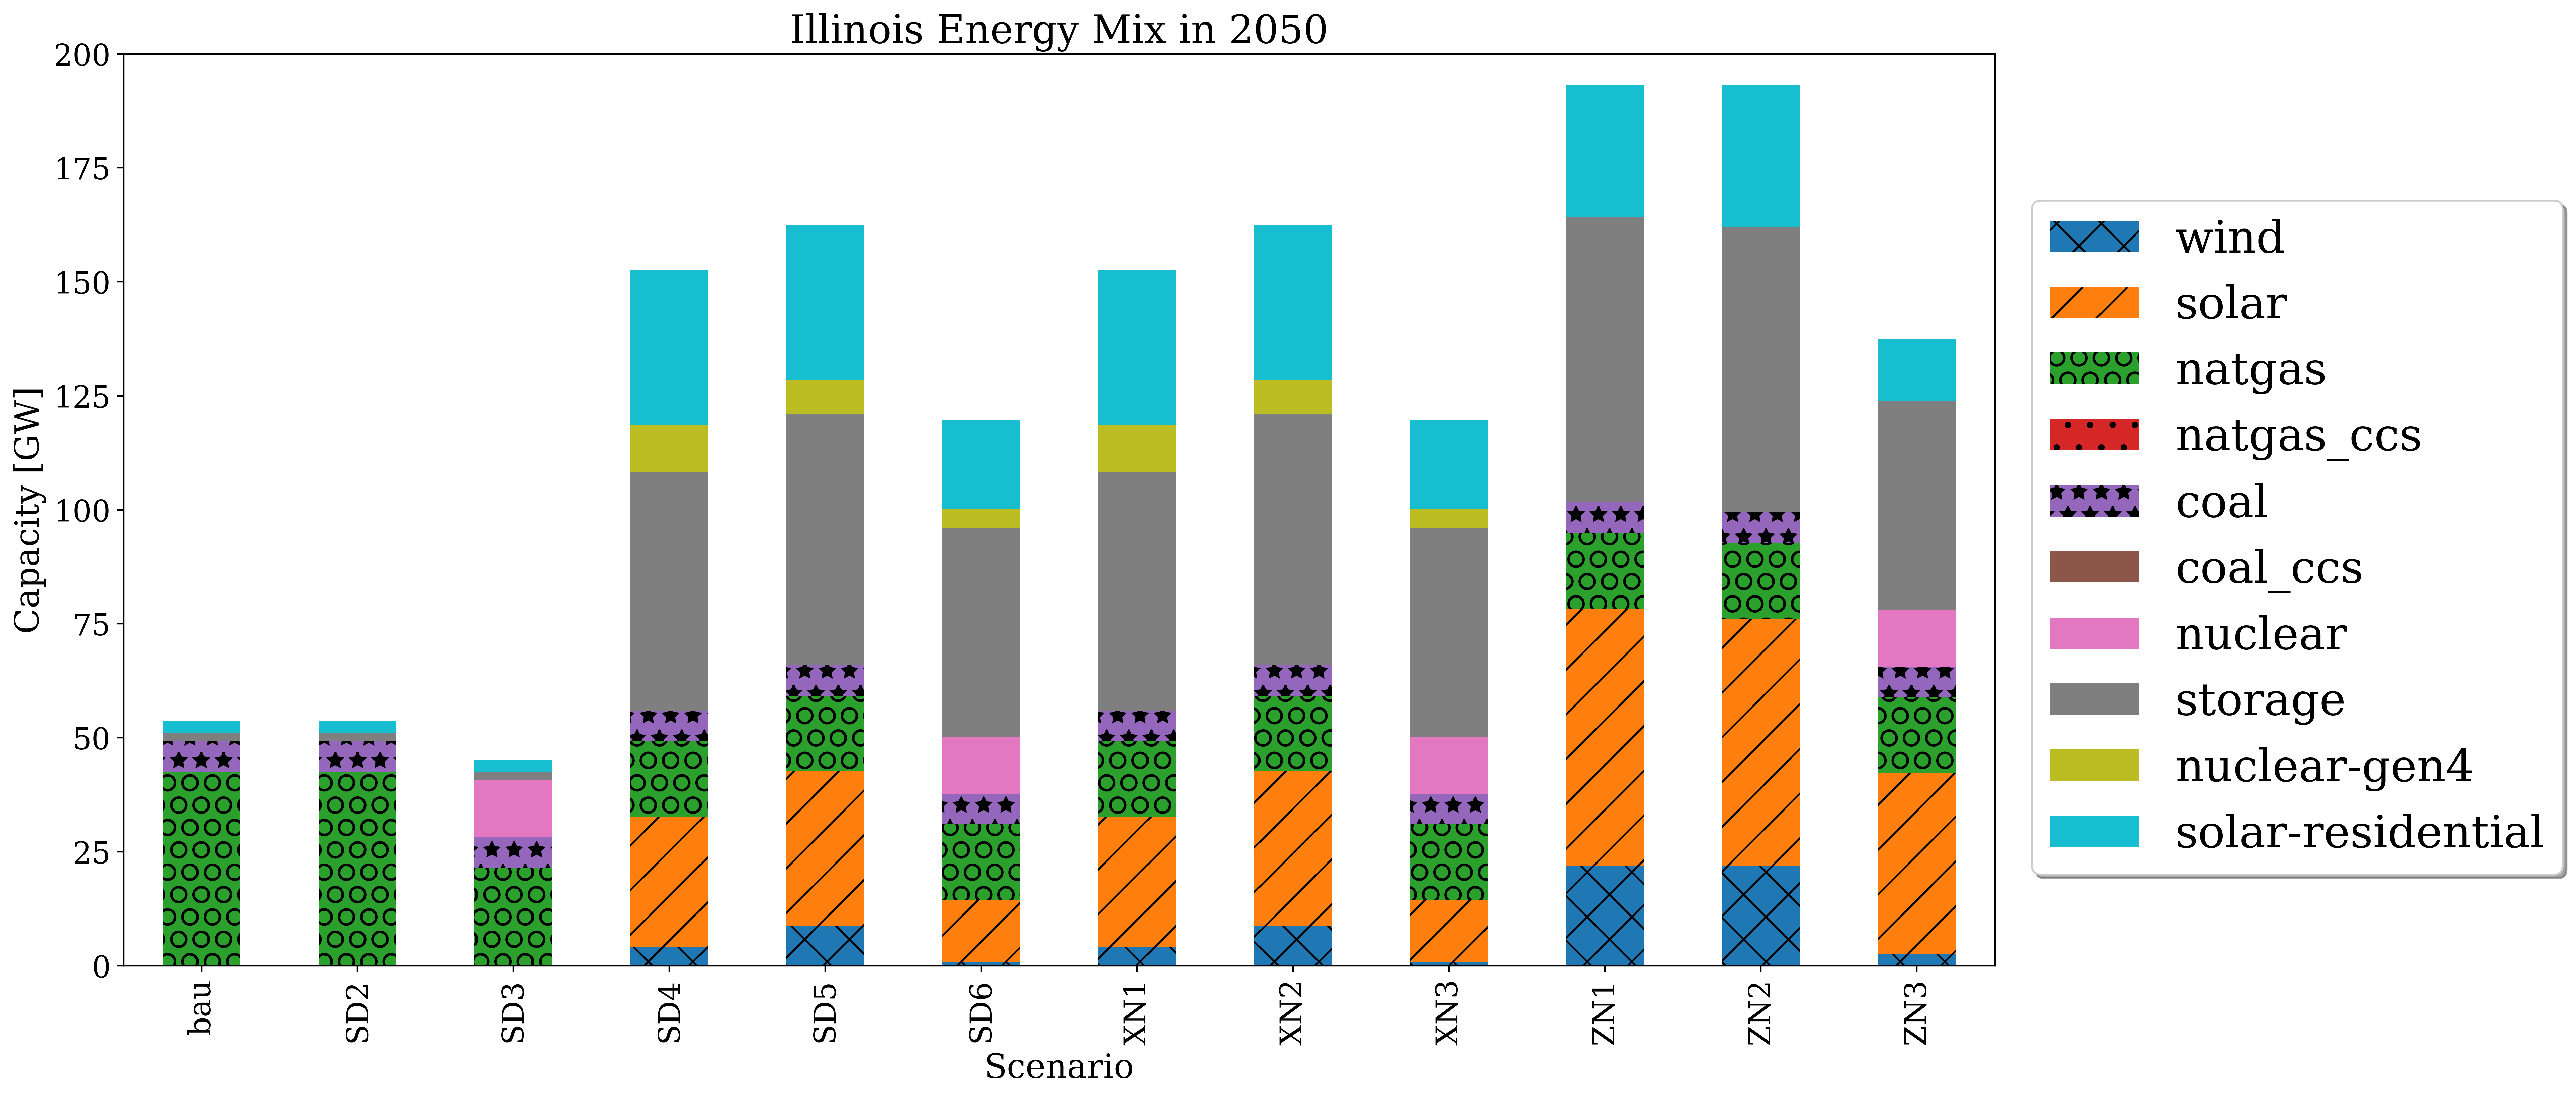
\includegraphics[width=\linewidth]{temoa/final_capacity.png}
  \caption{The mixture of electric generation in Illinois by 2050 for each scenario.}
  \label{fig:cap-2050}
\end{figure}

In the first two scenarios, BAU1 and BAU2, existing nuclear capacity is phased out
by 2050 and replaced almost entirely by natural gas capacity, without carbon
capture. A modest 2.7 GW of rooftop solar further displaces coal generation.
Existing wind turbines are also phased out by 2045 in these scenarios. In
scenario BAU3, all existing nuclear plants are maintained through 2050, halving
the required natural gas capacity.

Scenarios CC1, CC2, CC3, XN1, XN2, and XN3, simulate a strong climate policy by
forcing zero carbon emissions from electricity generation in 2030 and
aggressively pursuing renewable energy per the goals of the Clean Energy Jobs
Act \cite{illinois_clean_jobs_coalition_clean_2021}. However, even optimistic
deployment of renewable energy sources is insufficient to replace all of the
current coal and natural gas generation, let alone generation lost from
retiring nuclear plants. Advanced nuclear technology is required to achieve net-
zero carbon electricity generation by 2030 in each of these scenarios.

The final three scenarios, ZN1, ZN2, and ZN3, show the solar, wind, and battery
capacity required to replace electricity generation from all other technologies.
If the existing Illinois nuclear fleet is phased out, Illinois will have to
build 34 GW of rooftop solar, 77 percent of the technical limit \cite{gagnon_rooftop_2016}, along with 56 GW of utility scale solar by 2030.

In every scenario, Illinois will need, at minimum, 45.7 GW of 4.87 hour duration
energy storage to ensure grid reliability according to NERC recommendations
\cite{milligan_methods_2011}. With zero firm-capacity from nuclear
generation, 65.2 GW of battery storage is required.

\subsection{Total System Cost}
Figure \ref{fig:system-cost} shows the total system cost for each scenario.
All of the carbon-constrained scenarios are more expensive than business-as-
usual. In scenarios XN1, XN2, and XN3, which simulated significant cost overruns
for advanced nuclear technology, the total system cost is at most 0.06 percent
higher than in CC1, CC2, and CC3. Thus, the effect of cost overruns in new
nuclear builds is negligible. The ZNx scenarios are at most 5.5 percent cheaper
than scenarios with advanced nuclear. 

\begin{figure}[H]
  \centering
  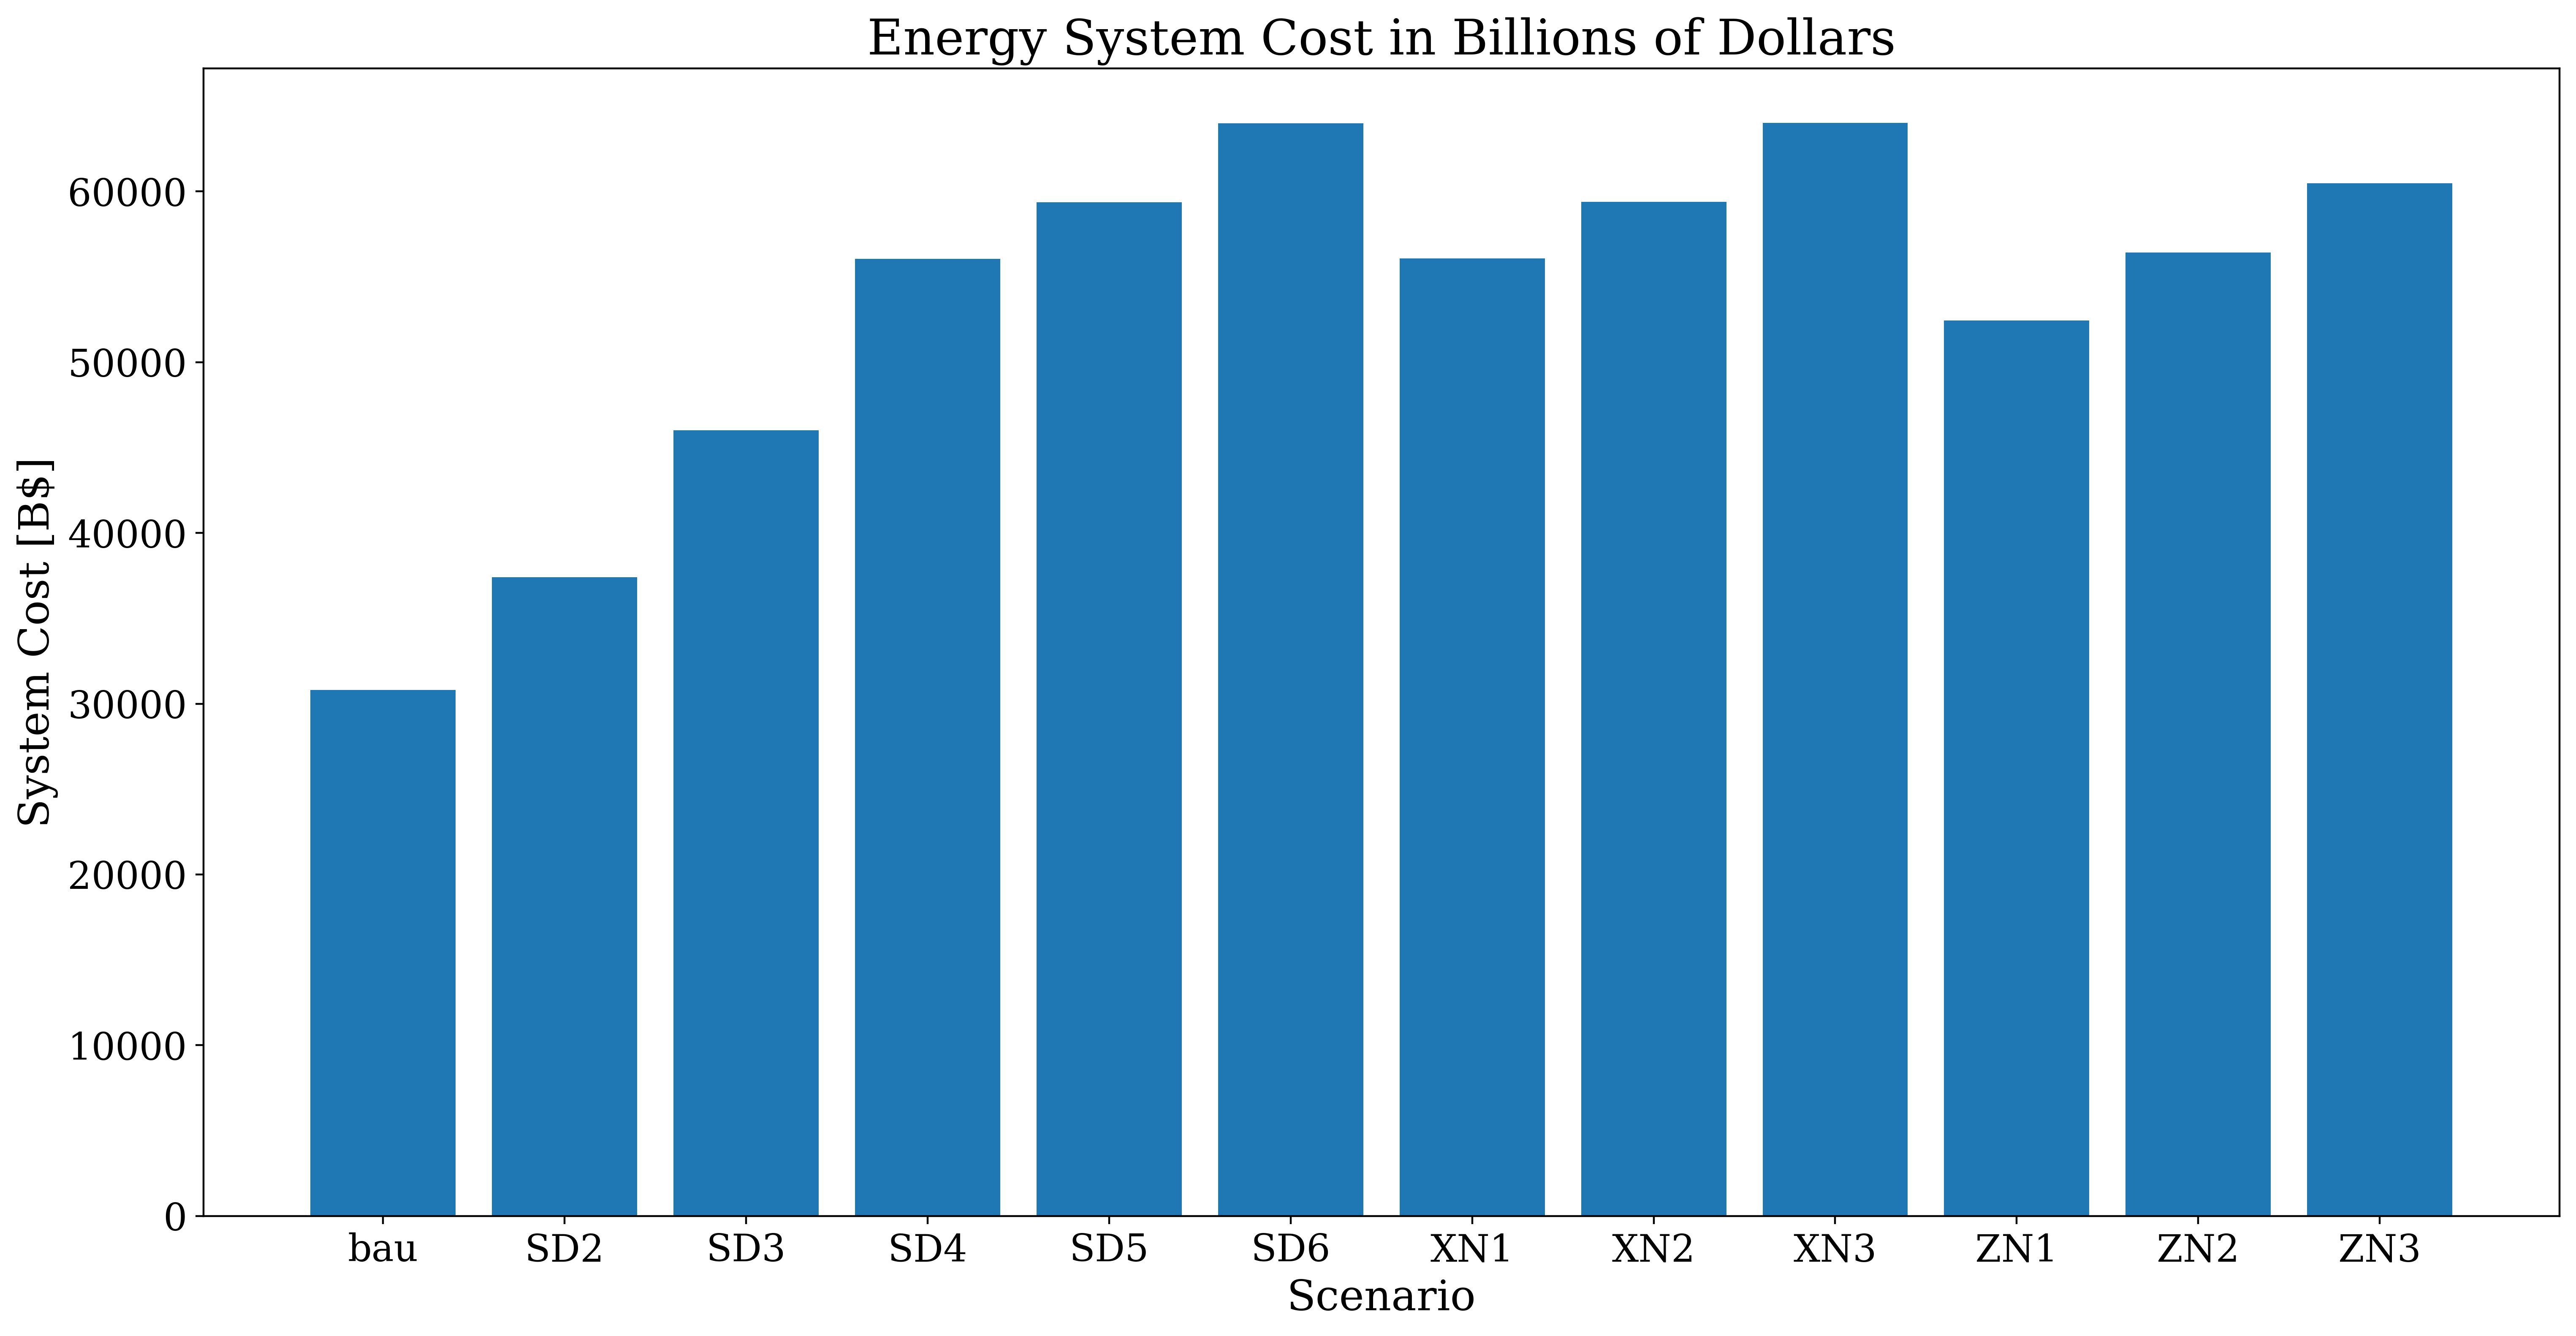
\includegraphics[width=\columnwidth]{temoa/total_system_cost}
  \caption{The total system cost for each scenario.}
  \label{fig:system-cost}
\end{figure}

\subsection{CO$_2$ Equivalent Emissions}

The lifecycle carbon equivalent emissions for each year in the simulation is
shown in Figure \ref{fig:co2eq-all} and the cumulative lifecycle emissions
for each scenario are shown in Figure \ref{fig:co2eq-cumulative}

\begin{figure}[H]
  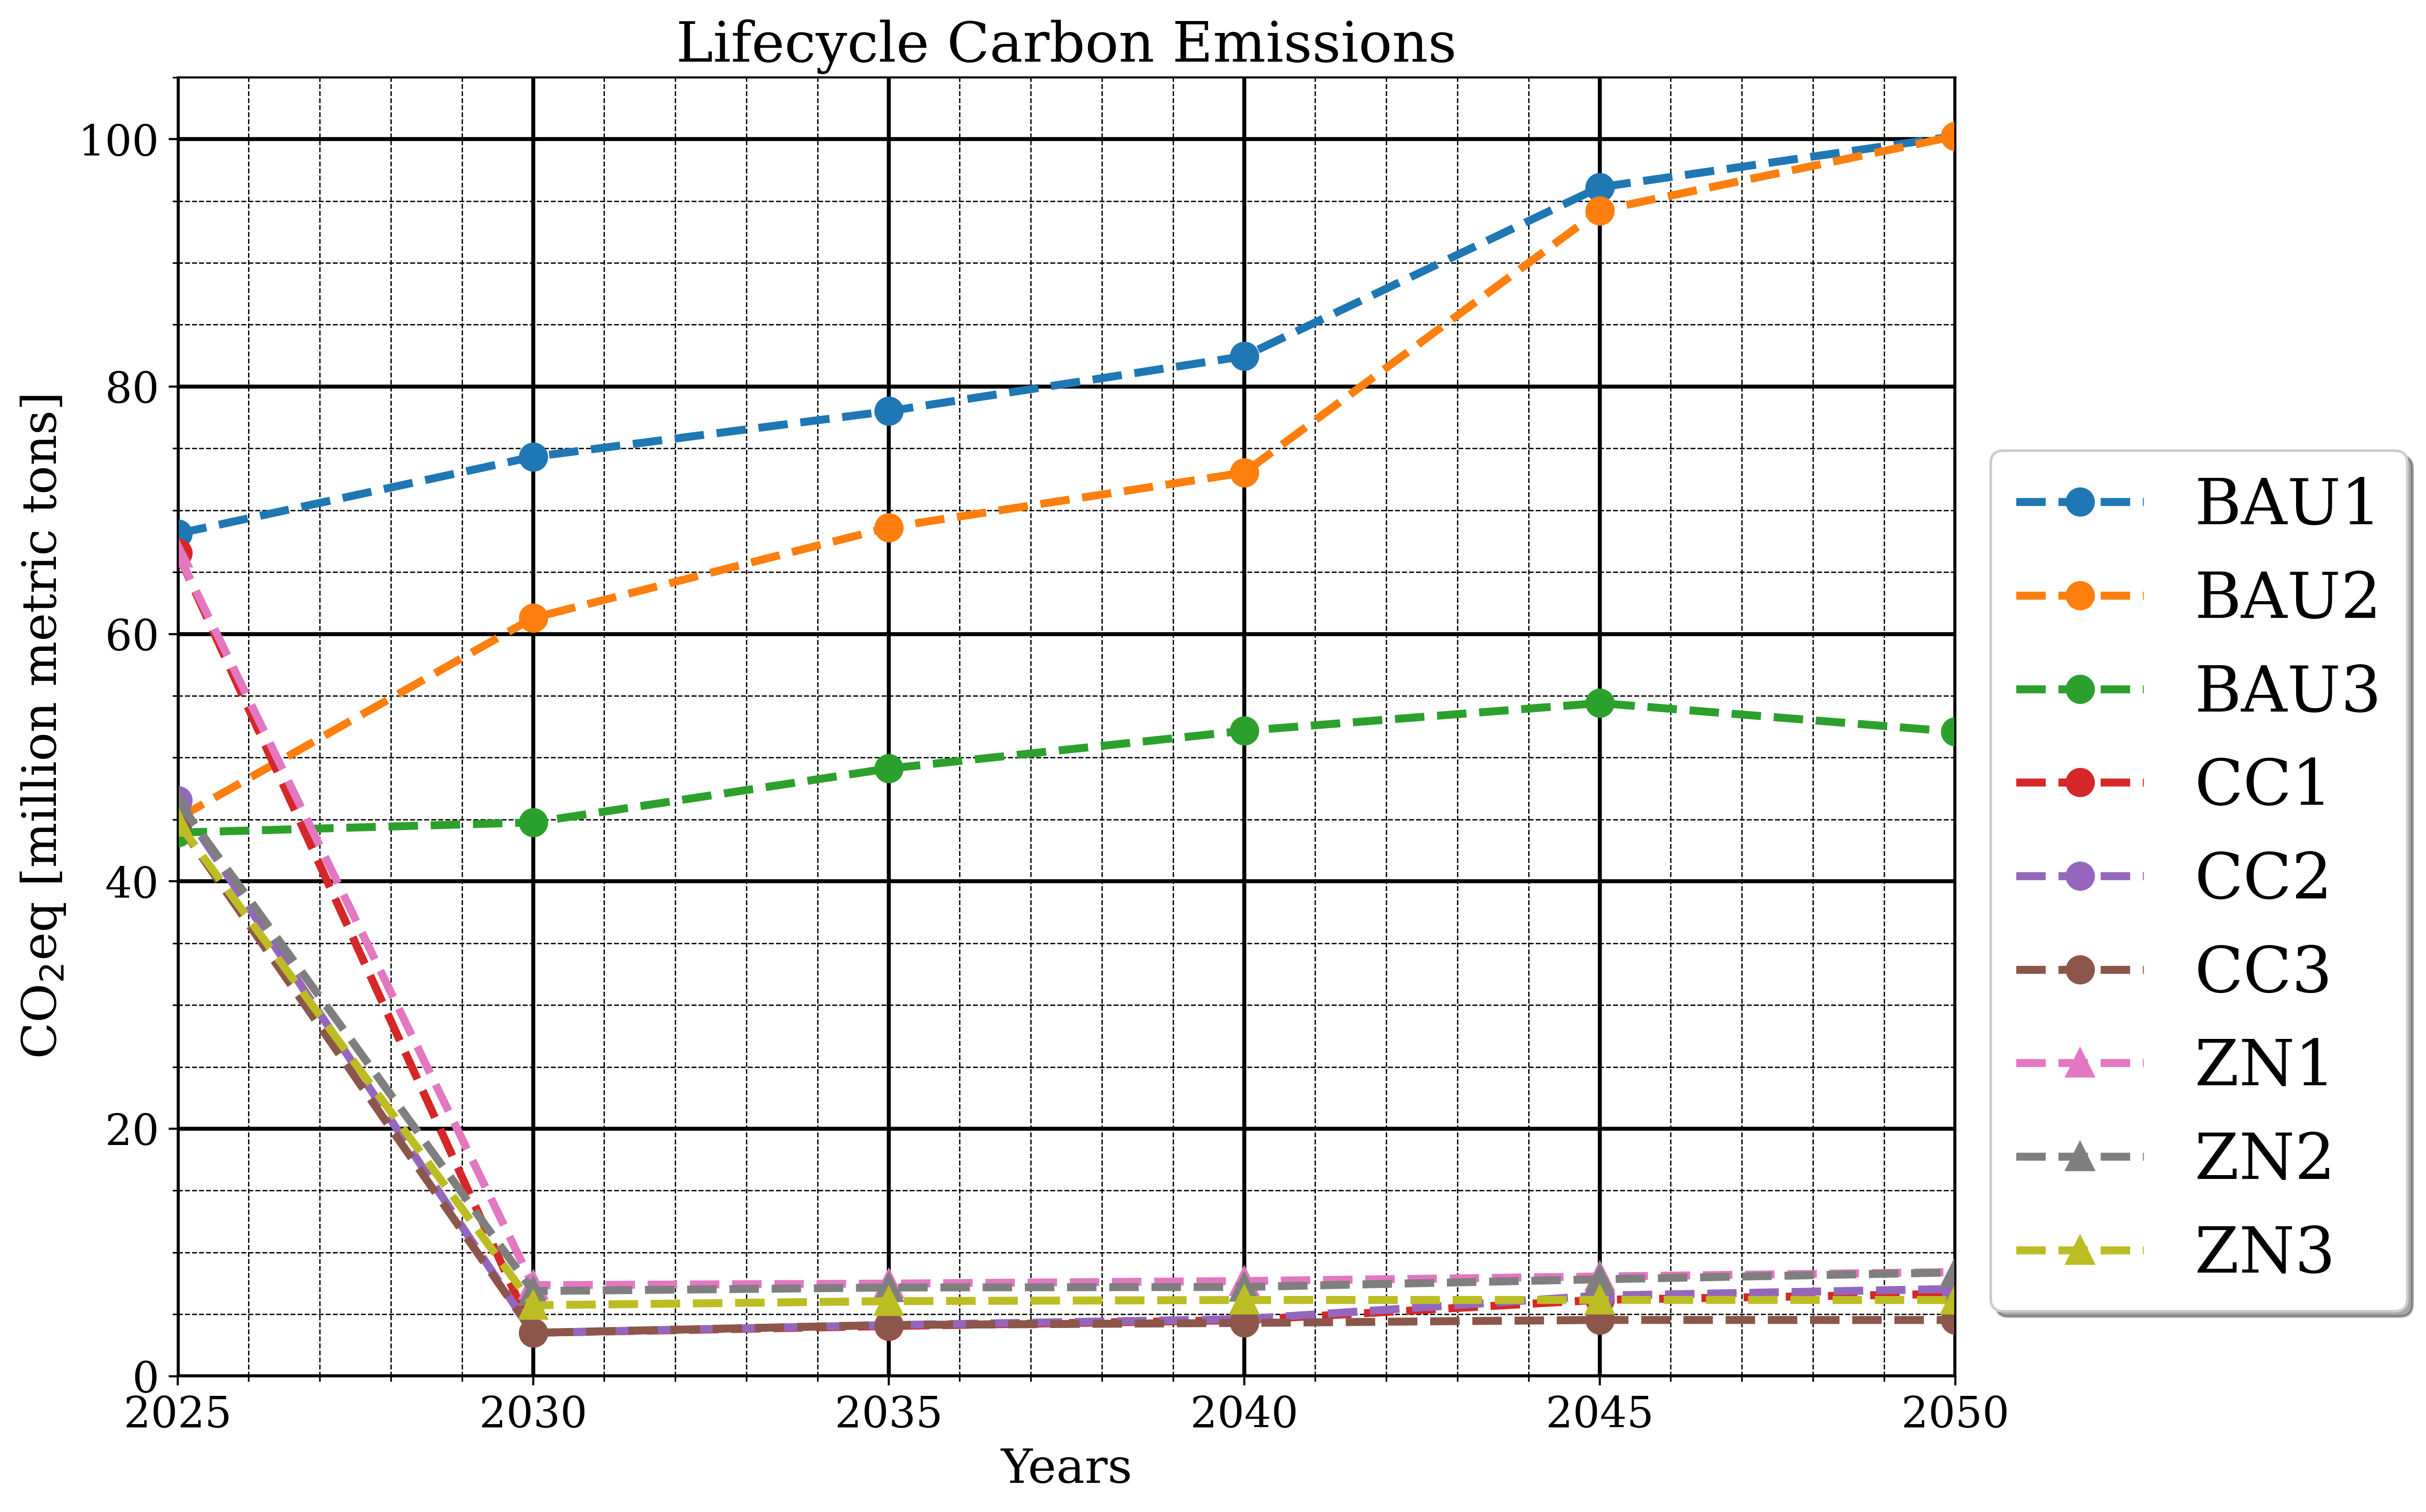
\includegraphics[width=\textwidth]{temoa/co2eq_all_comparison}
  \caption{A comparison of the lifecycle carbon equivalent emissions for
  each simulation year and across all scenarios.}
  \label{fig:co2eq-all}
\end{figure}

\begin{figure}[H]
  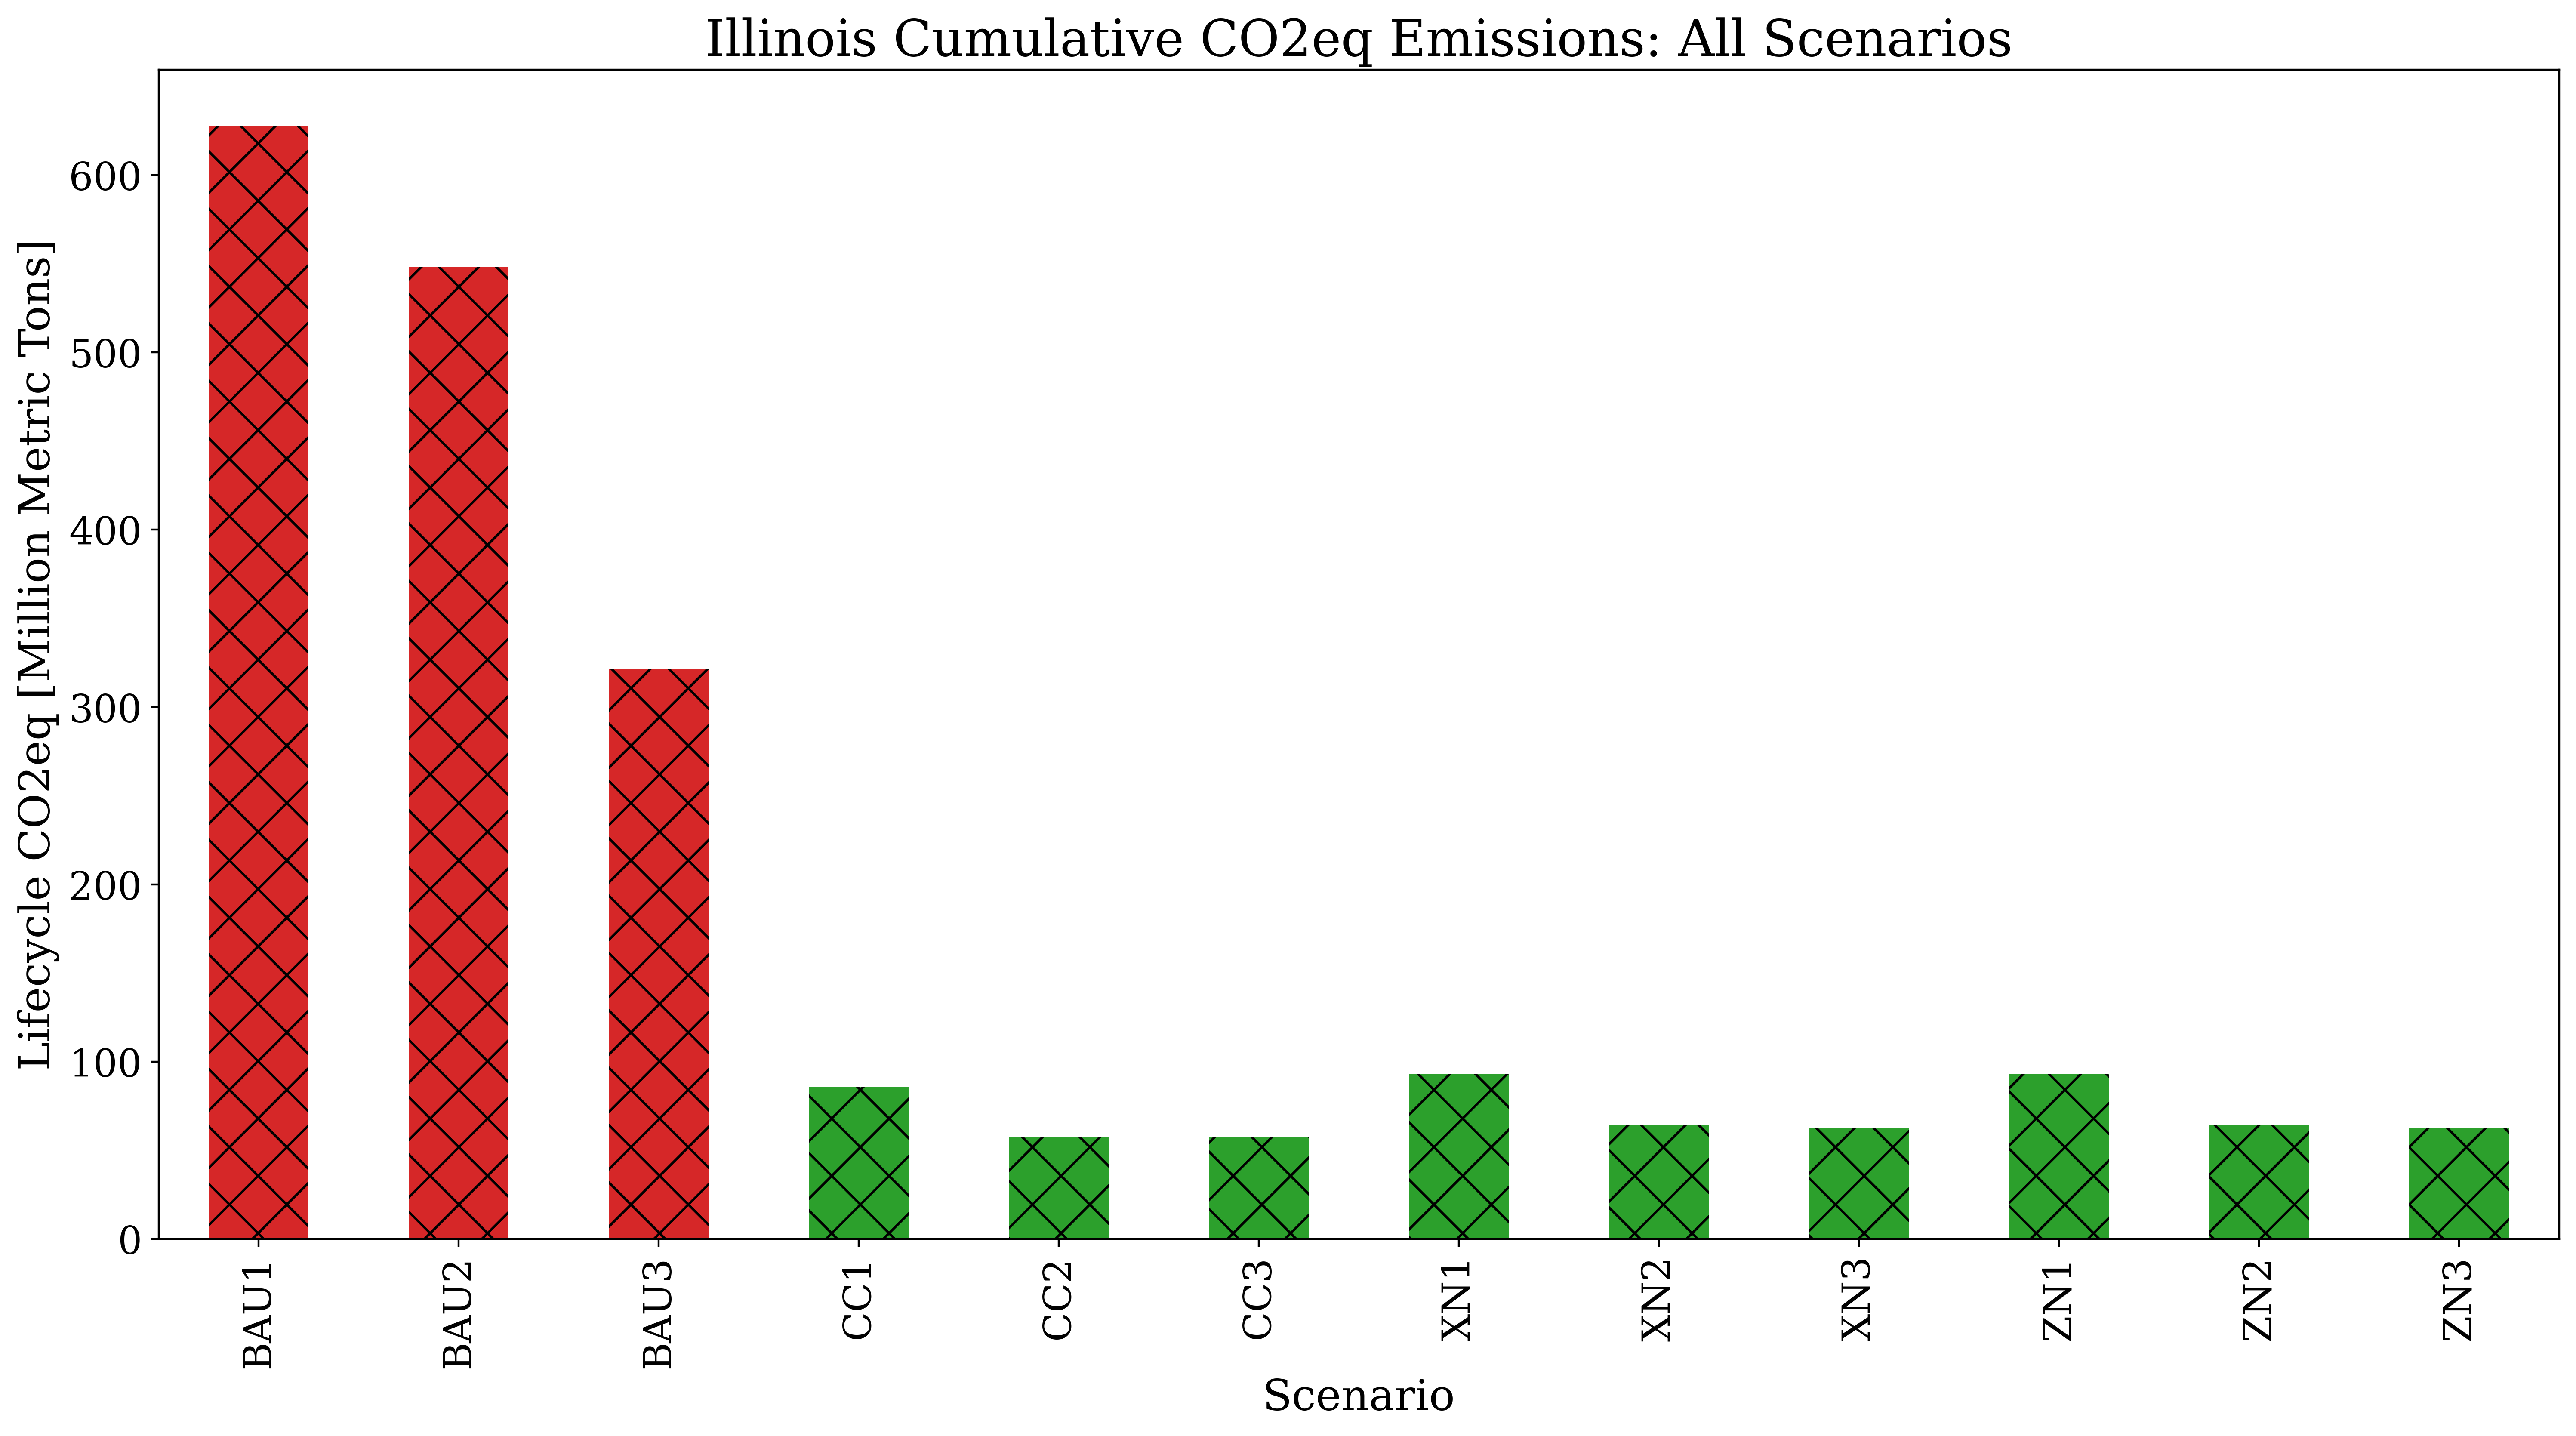
\includegraphics[width=\textwidth]{temoa/co2eq_all_comparison_barplot}
  \caption{A comparison of the total lifecycle carbon emissions in each
  scenario. Red bars denote scenarios without a carbon constraint. Green bars
  denote scenarios that constrained carbon emissions during operation.}
  \label{fig:co2eq-cumulative}
\end{figure}

Table \ref{tab:co2eq-cumulative} shows that keeping existing nuclear
plants open, while investing in both advanced nuclear technology and renewable
energy, generates the lowest lifecycle carbon emissions.

\begin{table}[H]
  \centering
  \caption{Cumulative Lifecycle CO$_2$eq Emissions\\The scenario with the
  lowest carbon emissions is in bold.}
  \label{tab:co2eq-cumulative}
  \begin{tabular}{lrc}
    \hline
    Scenario & CO$_2$eq & Existing Nuclear \\
    & [Million Tons]& Closures \\
    \hline
    BAU1 & 499.25& Premature\\
    BAU2 & 442.50& Scheduled\\
    BAU3 & 296.51& After 2050\\
    CC1/XN1 & 91.46 & Premature\\
    CC2/XN2 & 72.32& Scheduled\\
    \textbf{CC3/XN3} & \textbf{65.83}& \textbf{After 2050}\\
    ZN1 & 105.54& Premature\\
    ZN2 & 84.00& Scheduled\\
    ZN3 & 75.07& After 2050\\
    \hline
  \end{tabular}
\end{table}

\subsection{Solid Waste}

Solid waste forms are a key benefit of solar, wind, and nuclear technology since
society can decide how and where the waste will be stored or recycled. Figure
\ref{fig:total-waste} shows the total waste that must be handled by 2050.

\begin{figure}[H]
  \centering
  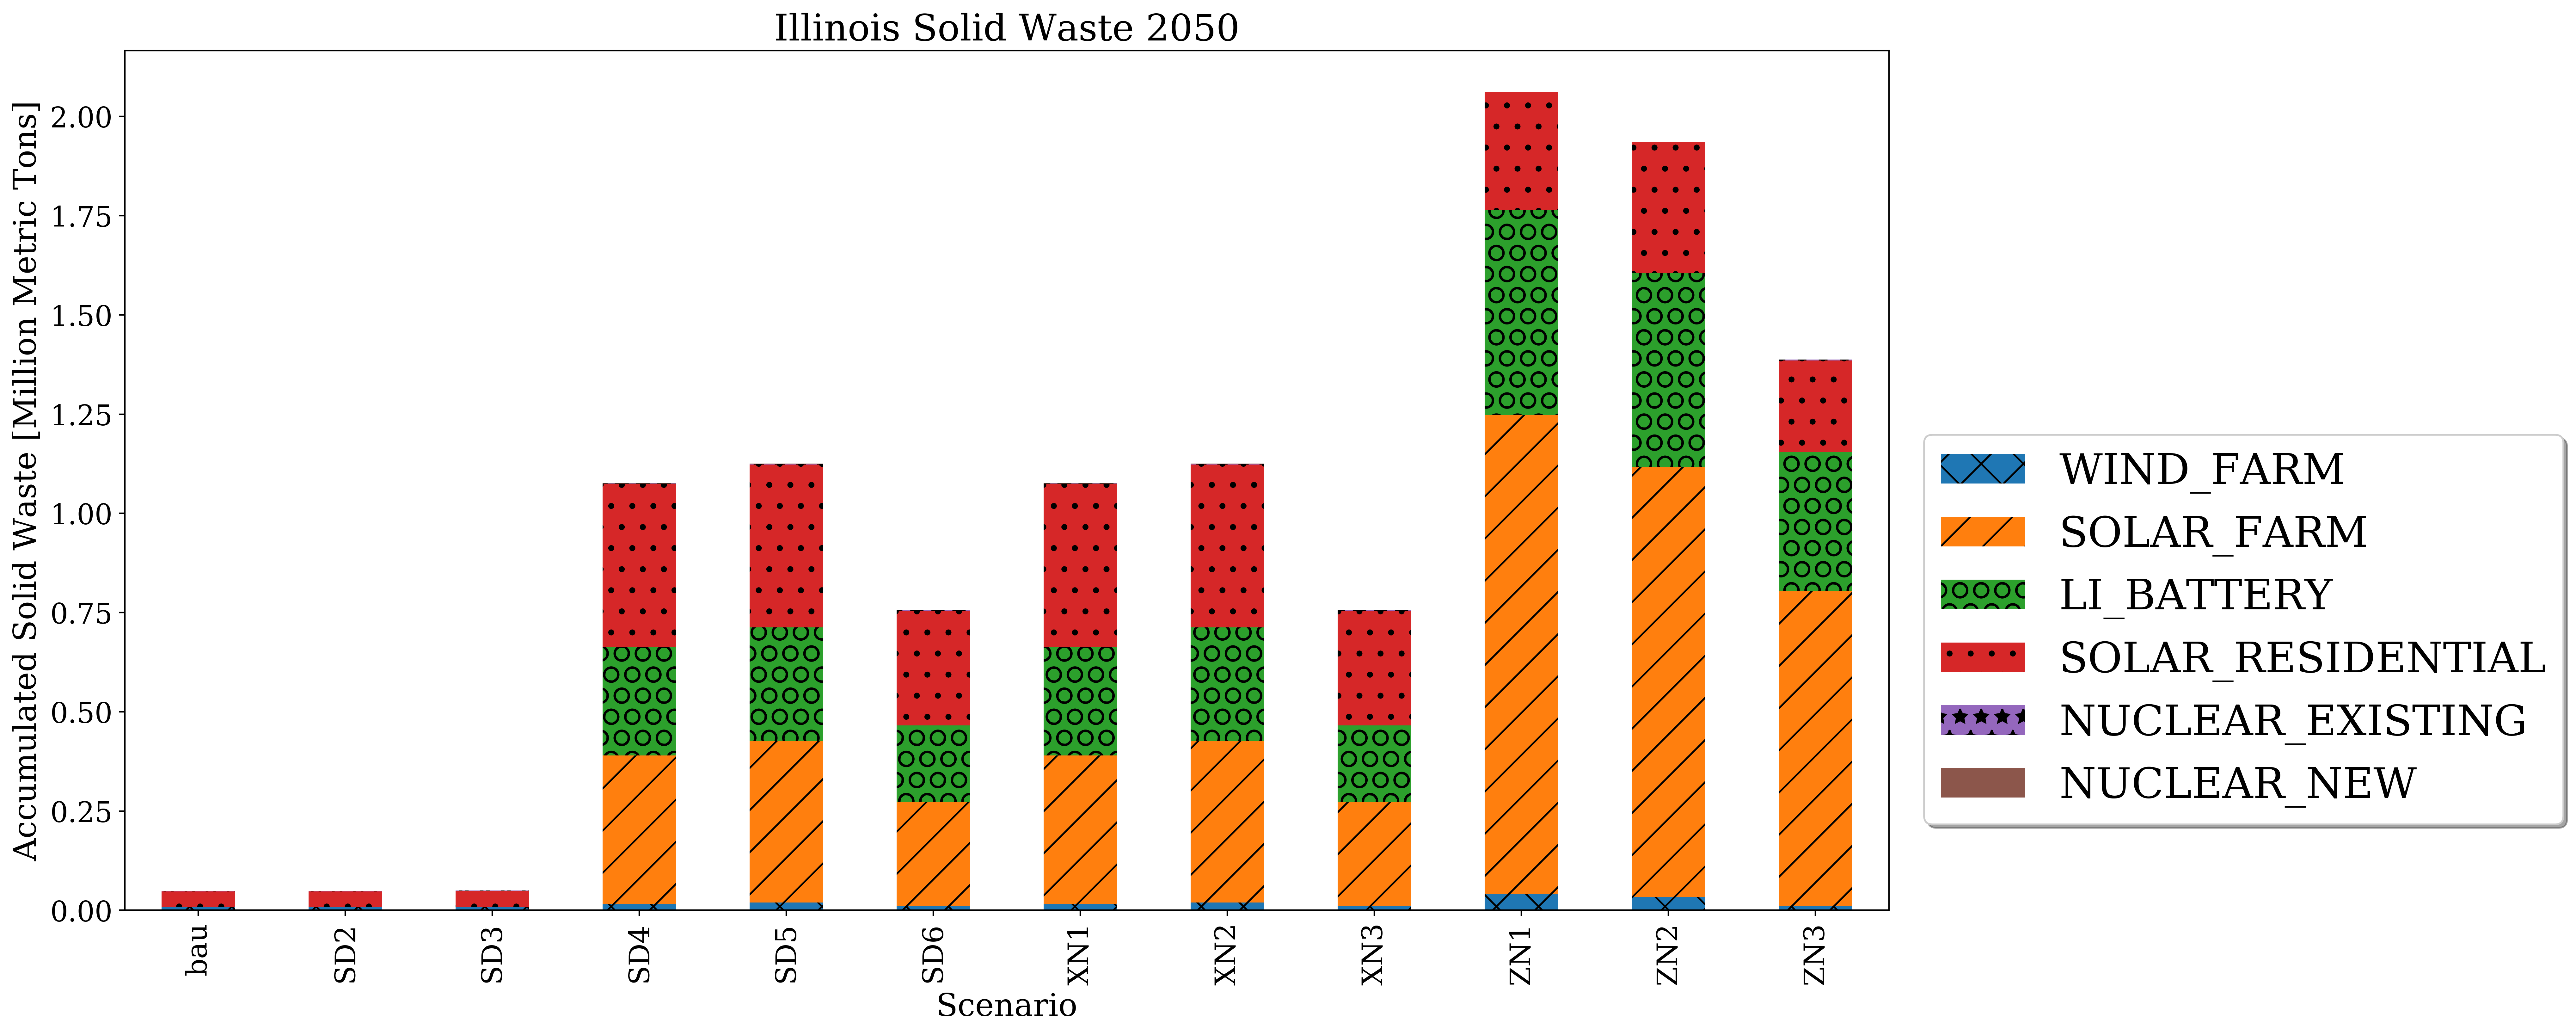
\includegraphics[width=\columnwidth]{temoa/total_solid_waste}
  \caption{The total solid waste accumulated from each clean technology by
  2050.}
  \label{fig:total-waste}
\end{figure}

The solid waste generated in scenarios BAU1, BAU2, and BAU3 are lower than all
other scenarios because most of the electricity generation in those scenarios
comes from fossil fuels. Which, of course, produces gaseous waste. Implicit to
handling solid waste are unmodeled energy and transportation requirements.
In every carbon-constrained scenario, keeping the existing nuclear plants open
through 2050 avoids the most solid waste production. Table \ref{tab:total-waste}
shows the total accumulated waste. Once again, the scenario that generates the
least solid waste is CC3/XN3, where the existing nuclear fleet is kept open,
renewable energy is built aggressively, and advanced nuclear technology is
pursued.

\begin{table}[H]
  \centering
  \caption{Solid Waste Accumulated by 2050\\The scenario with the
  lowest accumulated waste is in bold.}
  \label{tab:total-waste}
  \begin{tabular}{lrc}
    \hline
    Scenario & Solid Waste & Existing Nuclear \\
    & [Million Tons]& Closures \\
    \hline
    BAU1 & 0.0481& Premature\\
    BAU2 & 0.0485& Scheduled\\
    BAU3 & 0.0500& After 2050\\
    CC1/XN1 & 1.0765 & Premature\\
    CC2/XN2 & 1.1254& Scheduled\\
    \textbf{CC3/XN3} & \textbf{0.7569}& \textbf{After 2050}\\
    ZN1 & 2.0623& Premature\\
    ZN2 & 1.9363& Scheduled\\
    ZN3 & 1.3873& After 2050\\
    \hline
  \end{tabular}
\end{table}

\subsection{Land Use Change}

Land use is another important consideration for sustainable development. Figure
\ref{fig:land-use-percentage} shows the required land use in each scenario.
Conventional electricity generation requires very little land to operate due
to the high power density of those generators.

\begin{figure}[H]
  \centering
  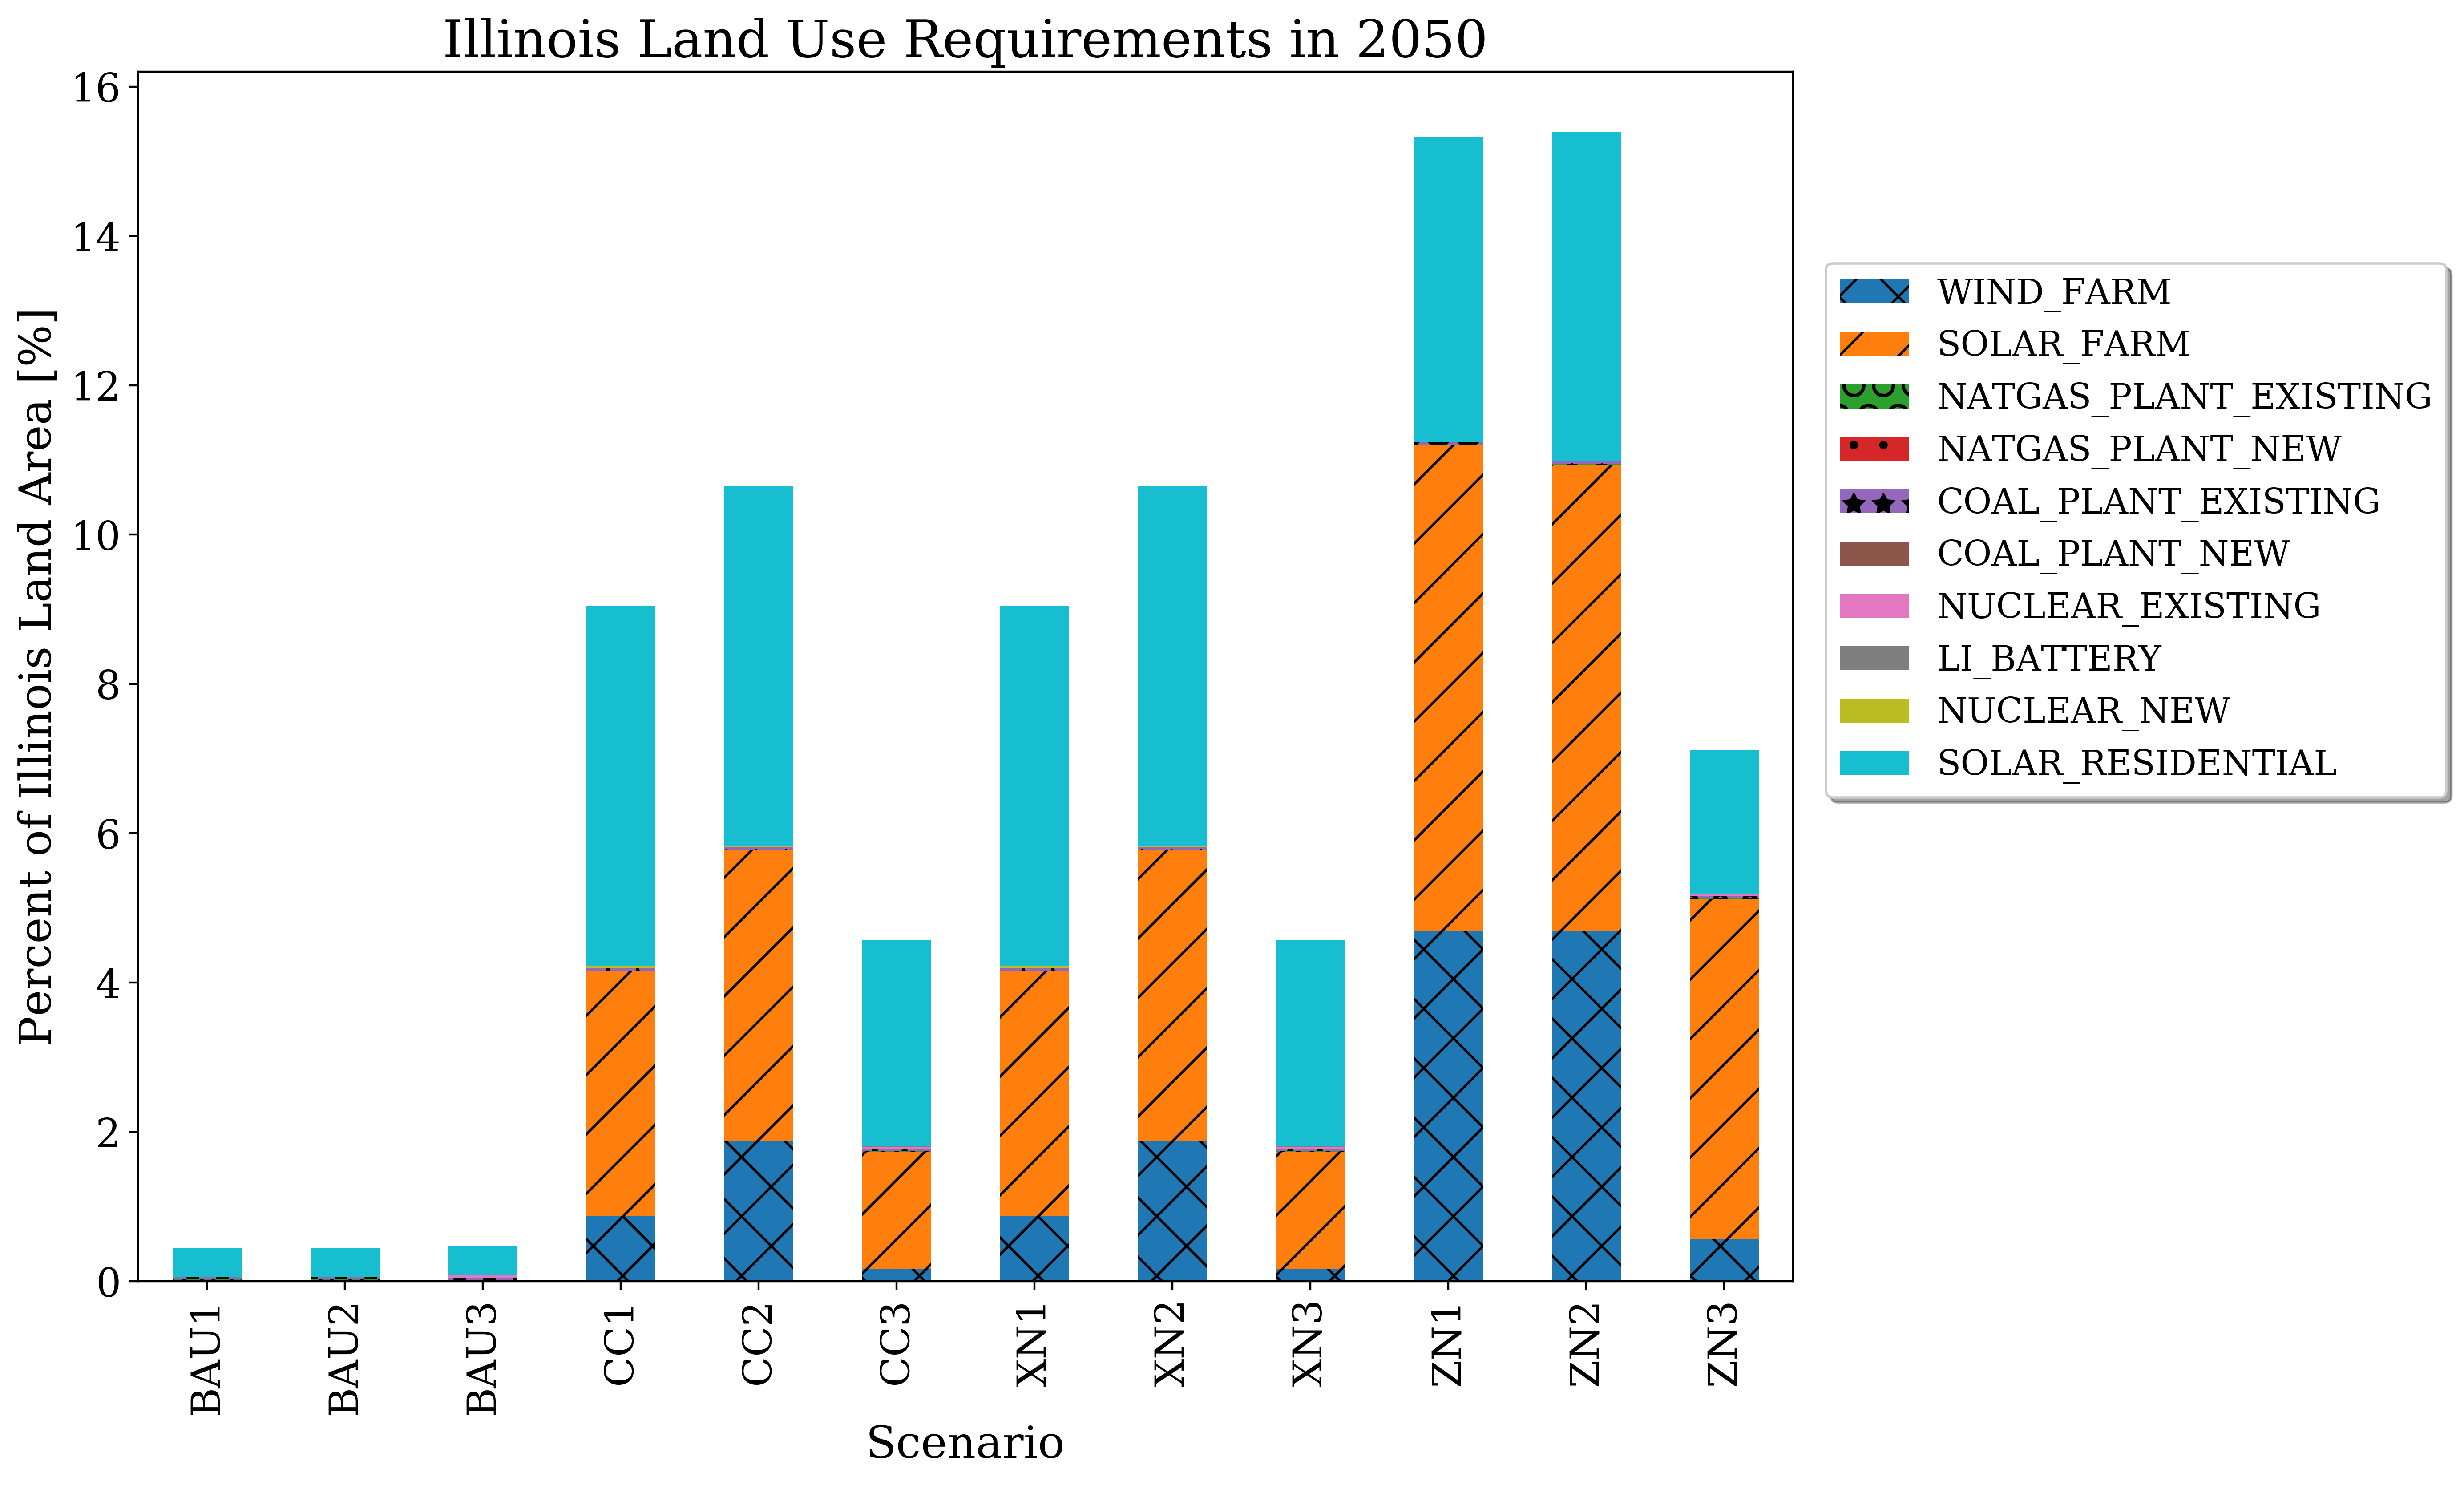
\includegraphics[width=\columnwidth]{temoa/total_landuse_percentage}
  \caption{The percentage of land use required for each scenario.}
  \label{fig:land-use-percentage}
\end{figure}

Table \ref{tab:land-use} shows the breakdown of land use change for each
renewable energy source as a percentage of Illinois' land area. In each of the
carbon-constrained cases, keeping the nuclear plants open through 2050 reduces
the land use change by half.

\begin{table}[H]
  \centering
  \caption{Land Use Requirements as a Percentage of Illinois' Area}
  \label{tab:land-use}
  \begin{tabular}{lrrrc}
    \hline
    Scenario & Wind Farms & Solar Farms & Rooftop Solar & Existing Nuclear \\
    & [\%]& [\%]& [\%]&Closures \\
    \hline
    BAU1 & 0.0000 & 0.0000 & 0.3891 &Premature\\
    BAU2 & 0.0000 & 0.0000 & 0.3891 &Scheduled\\
    BAU3 & 0.0000 & 0.0000 & 0.3891 &After 2050\\
    CC1/XN1 & 0.8687 & 3.2818 & 4.8227 &Premature\\
    CC2/XN2 & 1.8731 & 3.8973 & 4.8227 &Scheduled\\
    CC3/XN3 & 0.1676 & 1.5625 & 2.7486 &After 2050\\
    ZN1 & 4.6948 & 6.4962 & 4.0922 &Premature\\
    ZN2 & 4.6948 & 6.2401 & 4.4083 &Scheduled\\
    ZN3 & 0.5685 & 4.5510 & 1.9208 &After 2050\\
    \hline
  \end{tabular}
\end{table}

% =============================================================================
% =============================================================================
% =============================================================================
% =============================================================================
\begin{figure}[H]
	\centering
	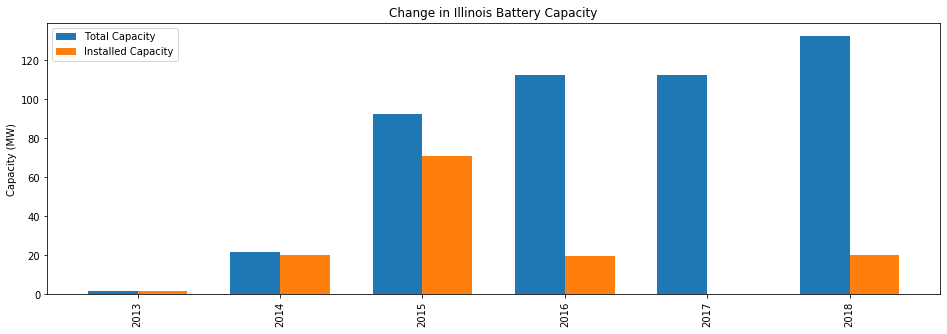
\includegraphics[width=\columnwidth]{./img/annual_installed_cap_battery.png}
	\caption{<++>}
	\label{fig:<++>}
\end{figure}


\begin{figure}[H]
	\centering
	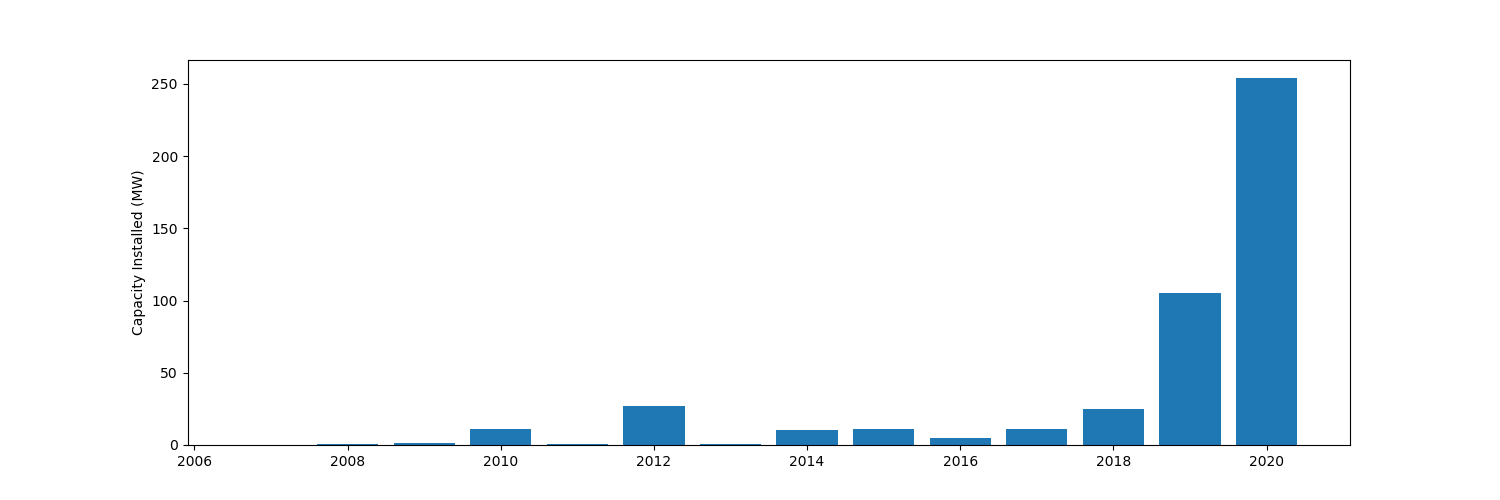
\includegraphics[width=\columnwidth]{./img/annual_installed_cap_solar.png}
	\caption{<++>}
	\label{fig:<++>}
\end{figure}


\begin{figure}[H]
	\centering
	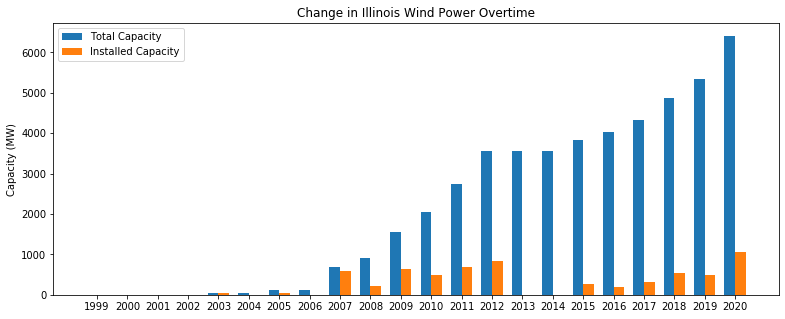
\includegraphics[width=\columnwidth]{./img/annual_installed_cap_wind.png}
	\caption{<++>}
	\label{fig:<++>}
\end{figure}


\begin{figure}[H]
	\centering
	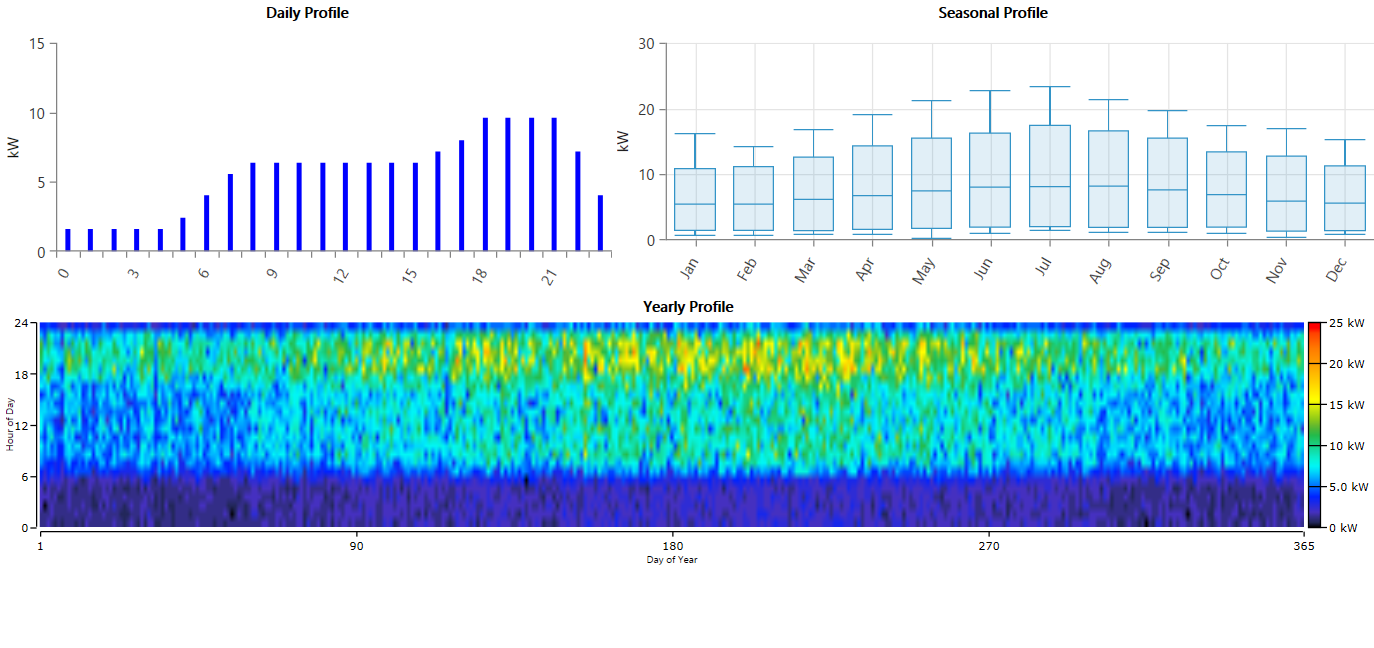
\includegraphics[width=\columnwidth]{./img/homer_illinois_loadprofile.png}
	\caption{<++>}
        \label{fig:<++>}
\end{figure}


\begin{figure}[H]
	\centering
	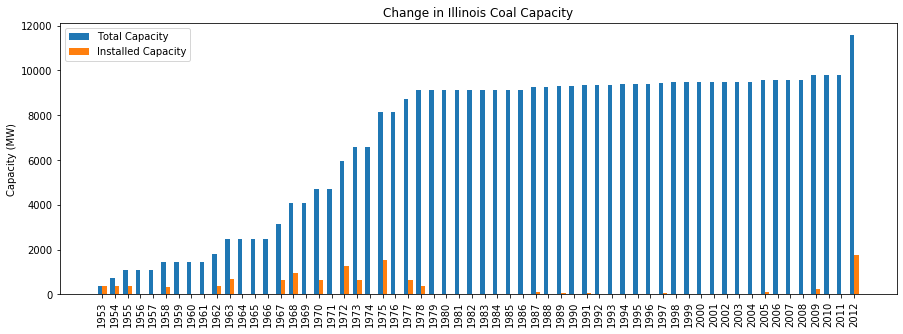
\includegraphics[width=\columnwidth]{./img/annual_installed_cap_coal.png}
	\caption{<++>}
	\label{fig:<++>}
\end{figure}


\begin{figure}[H]
	\centering
	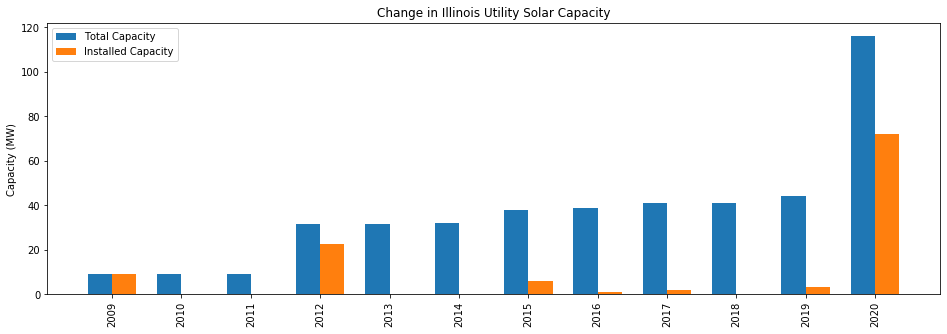
\includegraphics[width=\columnwidth]{./img/annual_installed_cap_utilityPV.png}
	\caption{<++>}
	\label{fig:<++>}
\end{figure}


\begin{figure}[H]
	\centering
	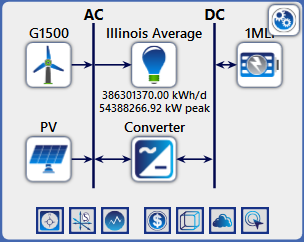
\includegraphics[width=\columnwidth]{./img/homer_system_setup.png}
	\caption{<++>}
	\label{fig:<++>}
\end{figure}


\begin{figure}[H]
	\centering
	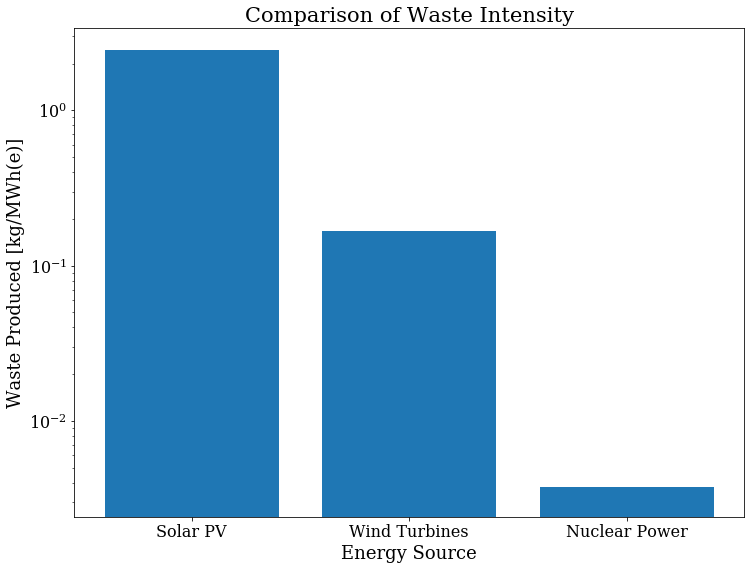
\includegraphics[width=\columnwidth]{./img/mass-waste-intensity.png}
	\caption{<++>}
	\label{fig:<++>}
\end{figure}


\begin{figure}[H]
	\centering
	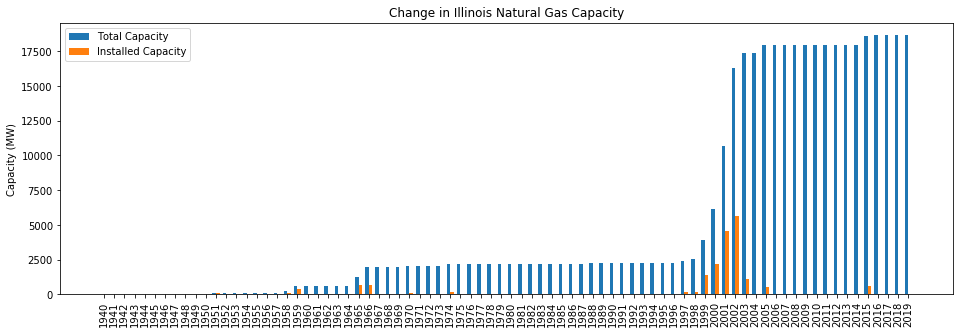
\includegraphics[width=\columnwidth]{./img/annual_installed_cap_natgas.png}
	\caption{<++>}
	\label{fig:<++>}
\end{figure}

\begin{figure}[H]
	\centering
	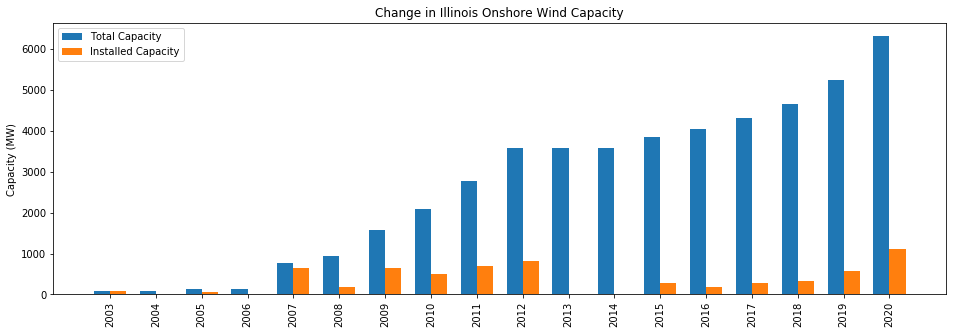
\includegraphics[width=\columnwidth]{./img/annual_installed_cap_utilitywind.png}
        \caption{<++>}
	\label{fig:<++>}
\end{figure}



\begin{figure}[H]
	\centering
        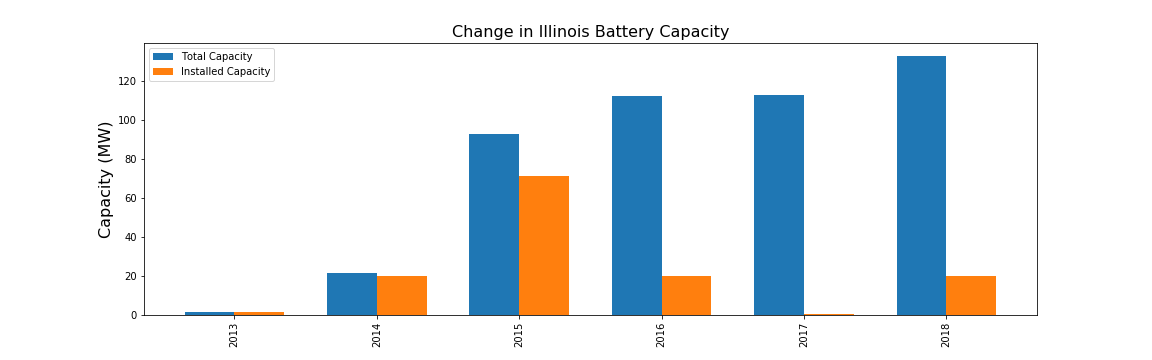
\includegraphics[width=\columnwidth]{./img/cap/battery.png}
	\caption{<++>}
	\label{fig:<++>}
\end{figure}

\begin{figure}[H]
	\centering
	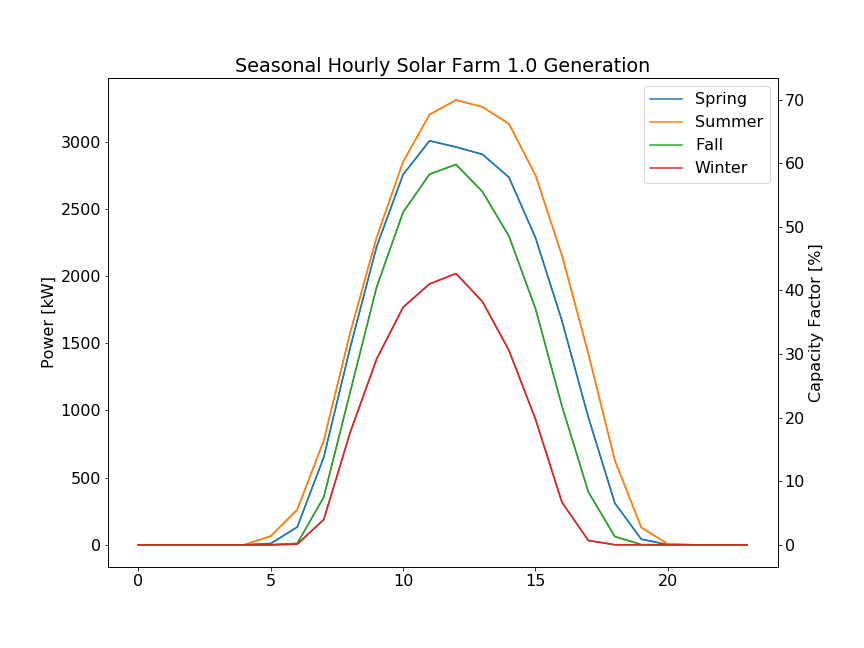
\includegraphics[width=\columnwidth]{./img/cap/seasonal_hourly_solar.png}
	\caption{<++>}
	\label{fig:<++>}
\end{figure}

\begin{figure}[H]
	\centering
	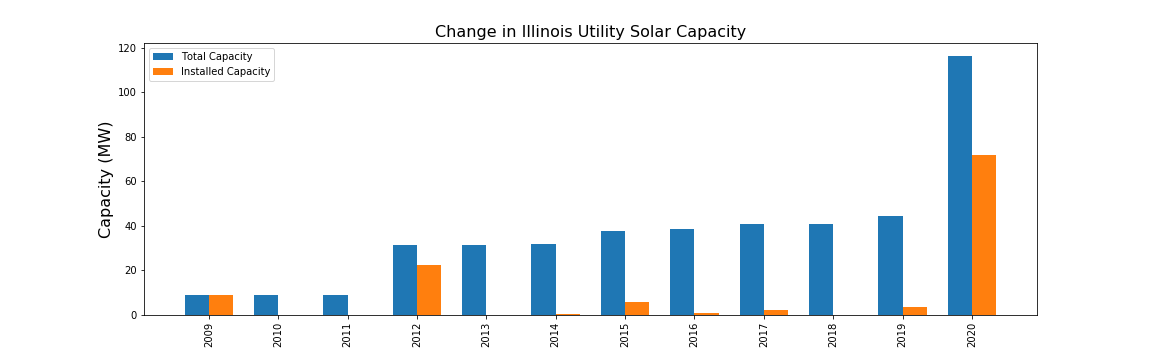
\includegraphics[width=\columnwidth]{./img/cap/solar.png}
	\caption{<++>}
	\label{fig:<++>}
\end{figure}

\begin{figure}[H]
	\centering
	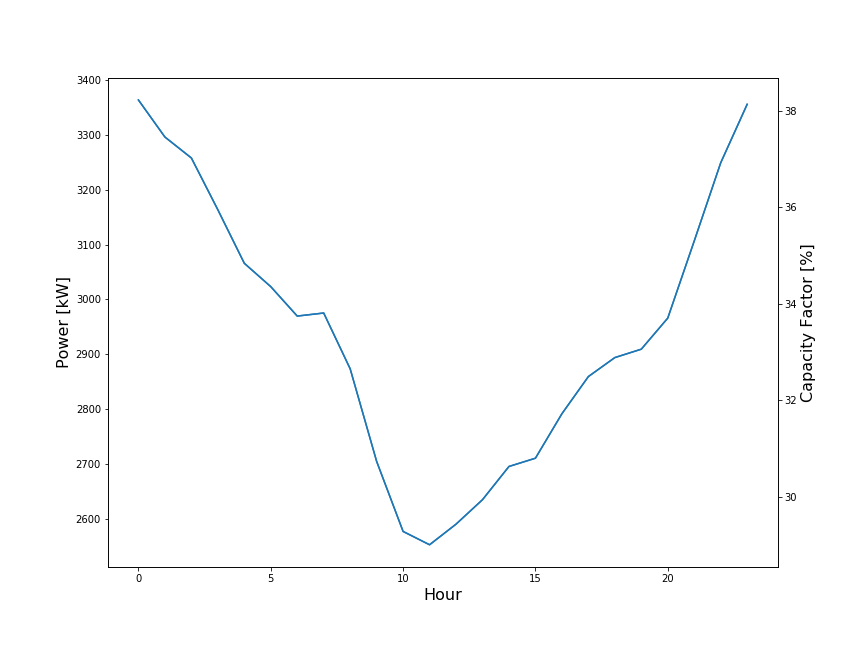
\includegraphics[width=\columnwidth]{./img/cap/wind_cf.png}
	\caption{<++>}
	\label{fig:<++>}
\end{figure}

\begin{figure}[H]
	\centering
	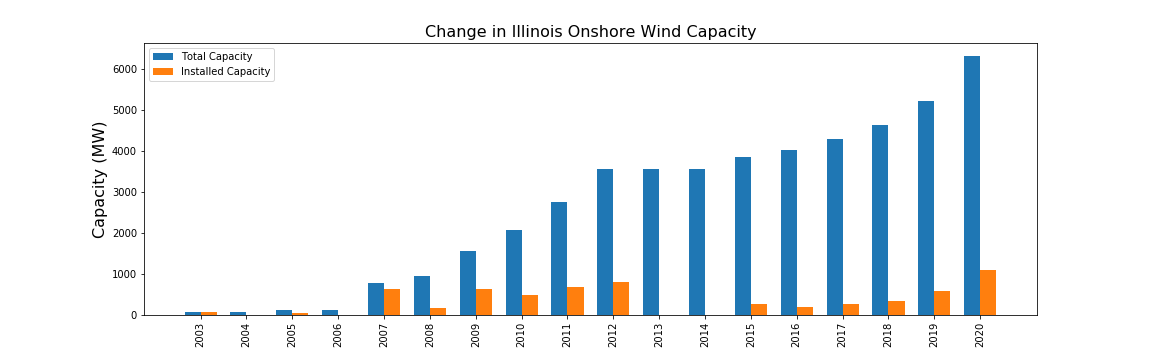
\includegraphics[width=\columnwidth]{./img/cap/onshore_wind.png}
	\caption{<++>}
	\label{fig:<++>}
\end{figure}

\begin{figure}[H]
	\centering
	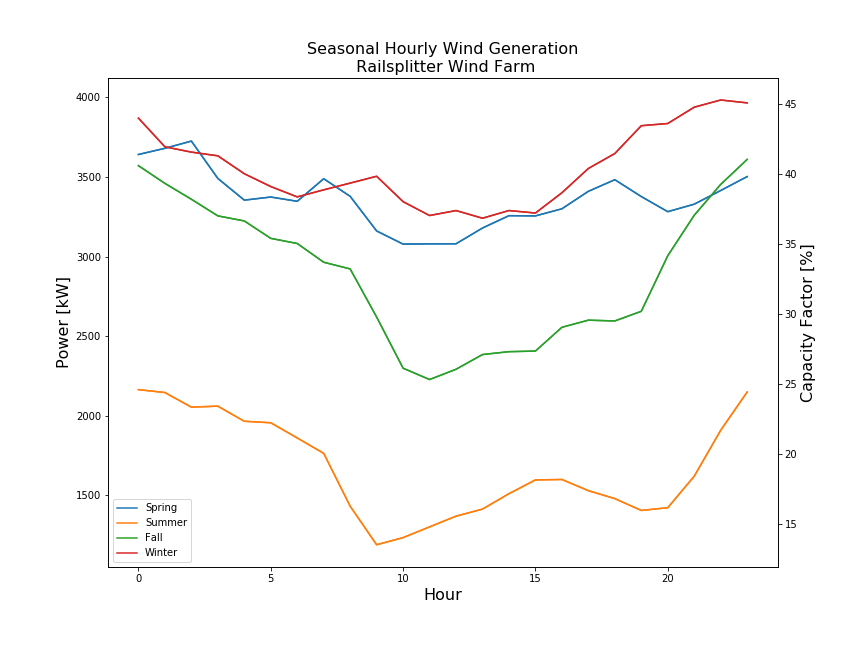
\includegraphics[width=\columnwidth]{./img/cap/seasonal_hourly_wind.png}
	\caption{<++>}
	\label{fig:<++>}
\end{figure}

\begin{figure}[H]
	\centering
	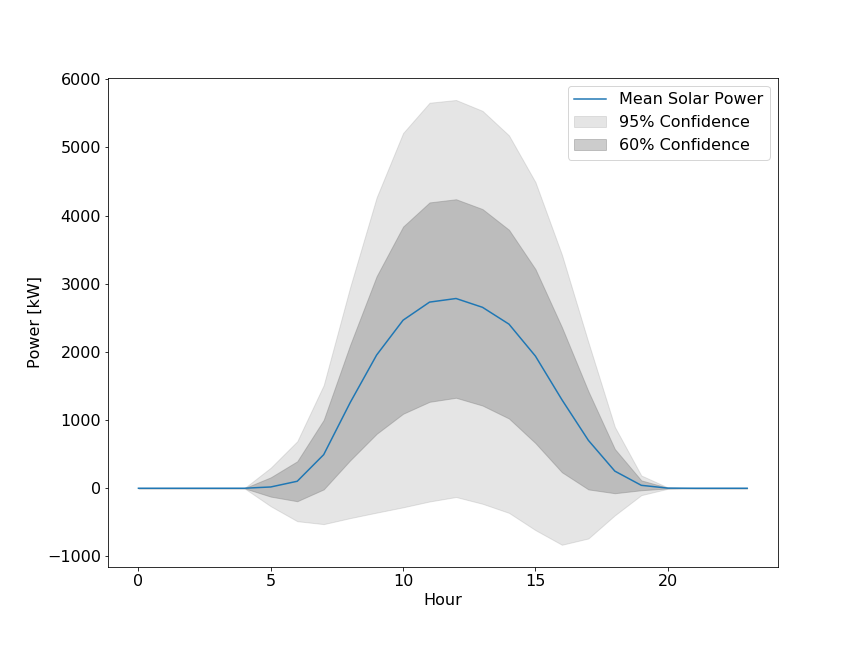
\includegraphics[width=\columnwidth]{./img/cap/solar_mean.png}
	\caption{<++>}
	\label{fig:<++>}
\end{figure}

\begin{figure}[H]
	\centering
	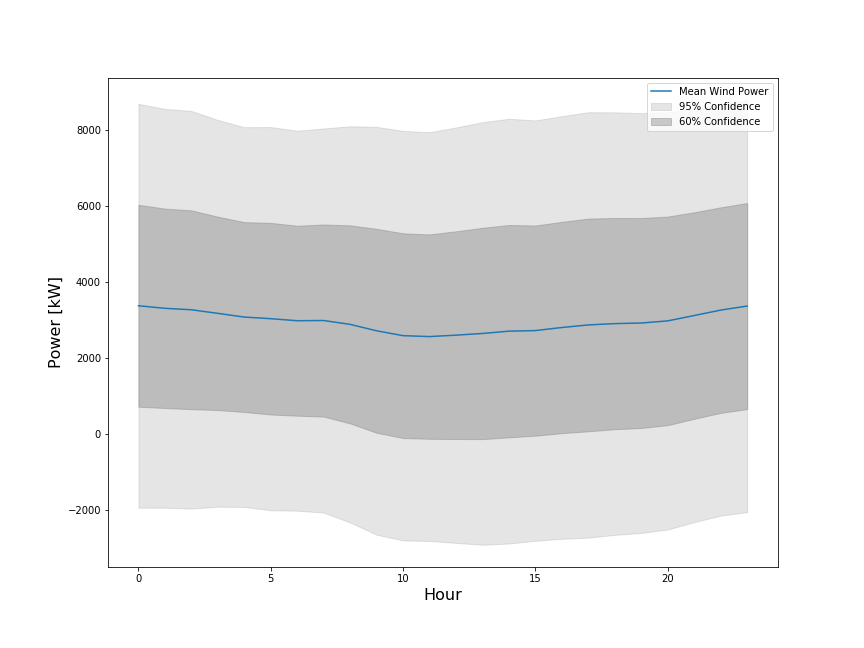
\includegraphics[width=\columnwidth]{./img/cap/wind_mean.png}
        \caption{<++>}
	\label{fig:<++>}
\end{figure}
